\chapter{Vorlesung 11}
\section{AVL-Bäume von Adelson-Velskii and Landis}


\begin{minipage}[t]{0.4\textwidth}
\begin{figure}[H]
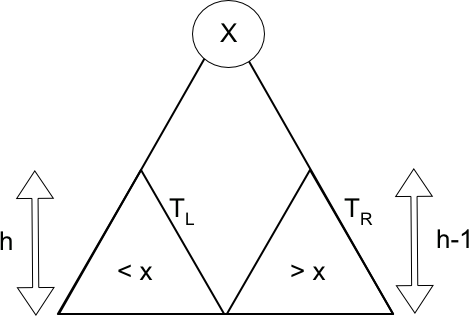
\includegraphics[width=\textwidth,left]{11/Grafik/img1.png}\\
\end{figure}
\end{minipage}%
%
\begin{minipage}[t]{0.55\textwidth}
\hspace{5mm}
\paragraph{Ziel:}%
Zeige, dass die maximale Tiefe eines AVL-Baums mit n Knoten ($\hat{=}~ n$ gespeicherten Schlüsseln) $O(\log(n))$ beträgt.\\
\end{minipage}


\underline{AVL-Eigenschaft:}\\ $|h(T_L)-h(T_R)| \leq 1$ muss für jeden Knoten des Baums gelten. $~~~\Rightarrow$ Suchzeit $O(\log(n))$ im worst case.\\
\newline

\begin{minipage}[t]{0.4\textwidth}
\begin{figure}[H]
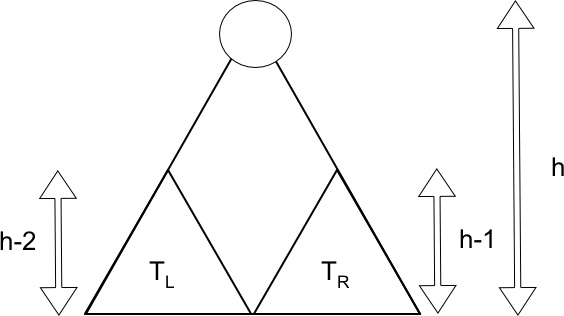
\includegraphics[width=\textwidth,left]{11/Grafik/img2.png}\\
\end{figure}%

\end{minipage}
\hspace{5mm}
\begin{minipage}[t]{0.55\textwidth}
$n(h) =$ minimale Anzahl von Knoten in AVL-Baum der Tiefe h\\

$n(h) \geq 1+n(h-2) + n(h-1)$ mit  $n(0)=0$ und $n(1)=1$\\

$n \geq f(h)^{\RM{1}} = \frac{1}{\sqrt{5}} \cdot (\phi^h-\phi^{-h})$ mit $\phi = \frac{1+\sqrt{5}}{2} \approx 1,61...$\\
$\Rightarrow n \geq c \cdot \phi^h$\\
$\Leftrightarrow h \leq \log{(\frac{n}{c})}$\\

$\Rightarrow h \in O(\log{n})$\\

$q.e.d$
\end{minipage}


\footnote[1]{$f(h)$ meint hierbei die h-te Fibonacci-Zahl} 

\pagebreak



\section{Rotationen}

\begin{figure}[H]
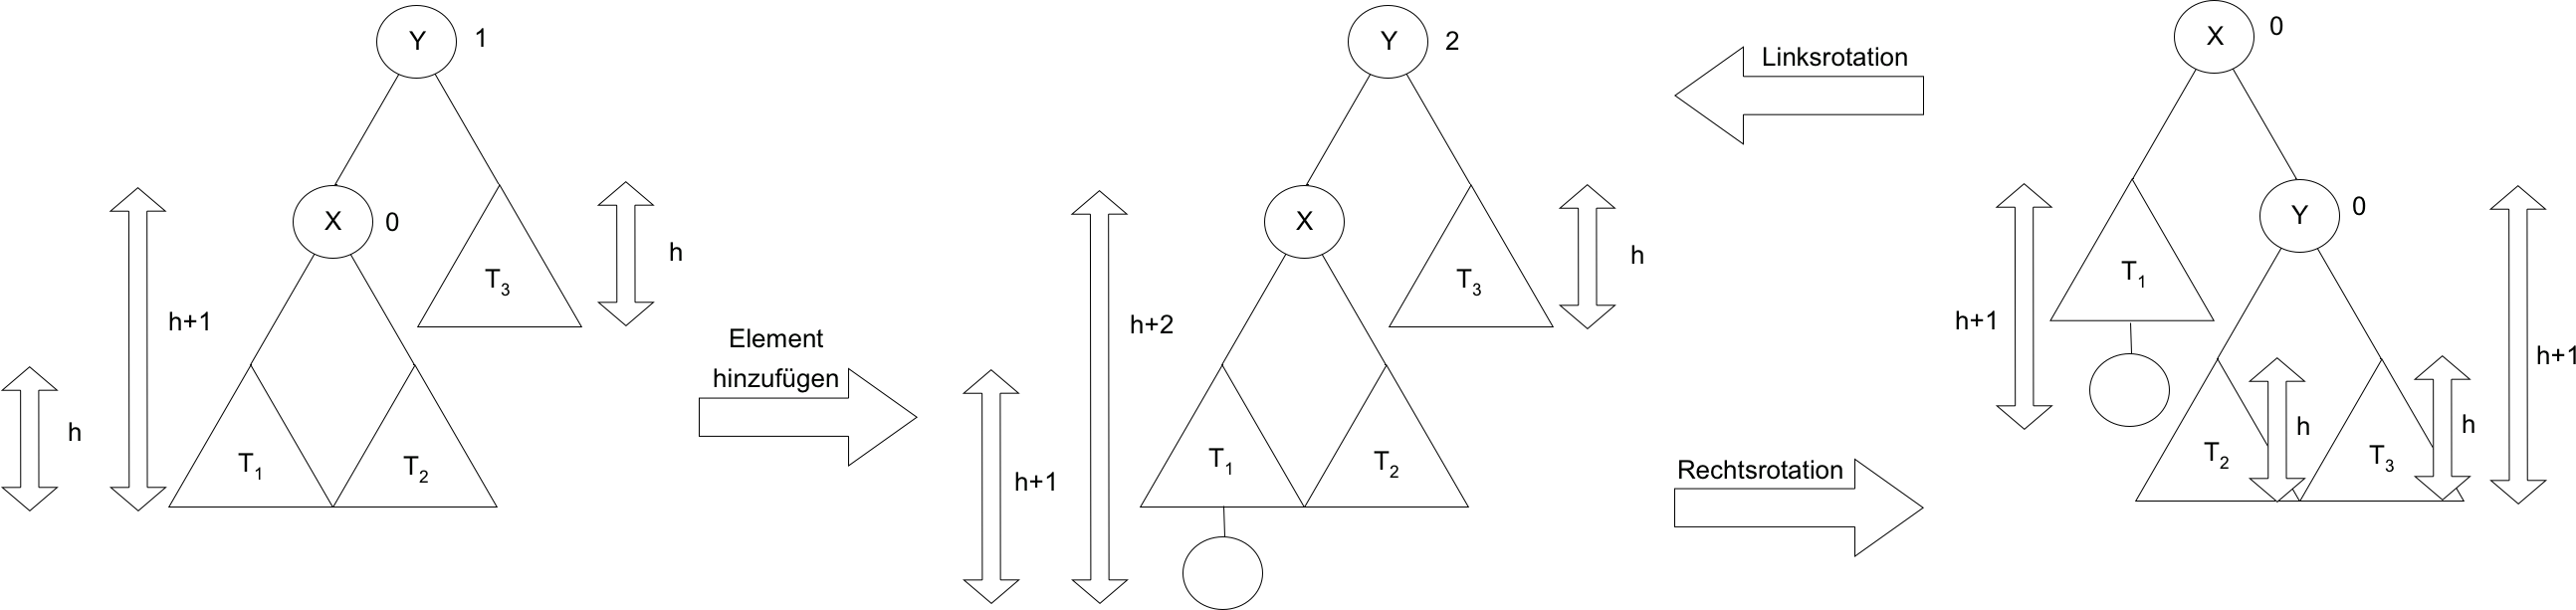
\includegraphics[width=\textwidth,left]{11/Grafik/img3_Rotation.png}\\

$Keys(T_1) \le Key(X) \le Keys(T_2) \le Key(Y) \le Keys(T_3)$ \\
\lstinline[language=Java]{balance(Y) = height(Y.left)-height(Y.right)}
\end{figure}



\pagebreak


\section{Pseudo-Code}
\lstinputlisting[language=Java]{11/Code/Node.java}

\paragraph{Anmerkung:} Die Laufzeit des Einfügens bleibt in $O($Baumtiefe$)$ = $O(\log{n})$. Nur einer der vier Fälle ist notwendig, um die Balance herzustellen. 
\pagebreak